\section{Литературный обзор}
\subsection{Постановка задачи}
   Разработать программный комплекс для анализа данных поверхностного ЭКГ-картирования. Далее задача подразделяется на две подзадачи.

Первый пункт -- разработать программу, которая будет прдставлять визуализацию результатов поверхностного ЭКГ-картирования.
Программе будет подаваться файл с числами (результатами обследования), и каждое число будет представлять определнный цвет. 
Для более красивого представления карты цветов будет использоваться интерполяция.

Второй пункт -- разработать систему для выявления у людей, страдающих ожирением скрытой эшемии.
Далее будет использоваться сокращенное название системы: <<ПКАДАД>>.
Система разрабатывается в компьютерной лаборатории МГИУ кафедры №11 для института питания РАМН в рамках договора о дружбе.
ПКАДАД будет применяться к пациентам, страдающих ожирением различных степеней.
Сначала, пациент, проходит тест на аппарате \verb|Astrocard|.
Затем следует считывание данных на различных стадиях: пик, покой на первой, третьей, пятой и седьмой минутах.
После обработки всех данных, программа должна дать ответ на вопрос: «Есть ли скрытая эшемия или нет?».


\subsection{Анализ подобных систем}
При анализе подобных систем было выявлено, что требуемой системы не существует.
Данный комплекс будет разрабатываться впервые.

\subsection{Выбор архитектуры программного обеспечения}
ПКДАД будет разрабатываться на базе WINDOWS 8 с использованием библиотеки QT версии 5.0.2.
Языком программирования был выбран язык c++. Также будет задействована библеотека OPEN GL.


\subsection{Задачи, которые требуется решить}
\begin{itemize}
\item Сжатие результатов обследования при помощи анализа главных компонент.
Одна из самых масштабных задач. Т.к. файлы экспорта имеют достаточно
большой размер, превышающий 300 мегабайт. Предварительное сжатие файла,
позволит сократить его объем до 15 мегабайт. Данная процедура, в
дальнейшем, существенно ускорит работу программы. Анализ главных
компонент - один из основных способов, позволяющих сократить размерность
данных, при котором у нас происходит минимальная потеря количества
информации.
\item Разработка интерфейса для ввода данных и формирования групп пациентов.
Интерфейс будет разрабатываться при помощи библиотеки QT версии 5.0.2.
\item Обучение нейронной сети(многослойный персептрон).
\item Тестирование нейронной сети и анализ полученных данных. Изучение
структуры многослойного персептрона в зависимости от результатов
(Настройка нейронной сети).

\newpage
\subsection{Объекты автоматизации}
\begin{figure}[ht!]
\begin{center}
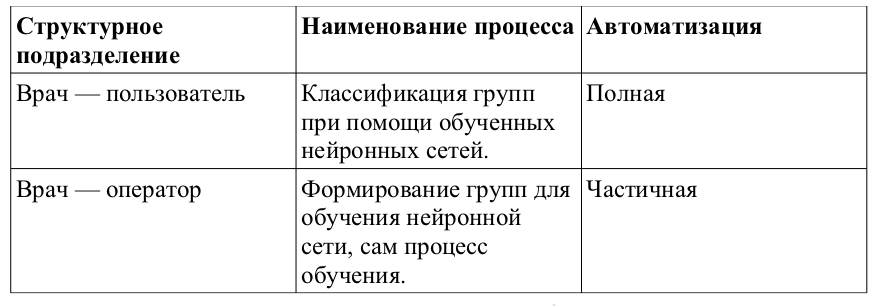
\includegraphics[scale=0.5]{ris3}
\end{center}
\end{figure}

\item Классификация групп при помощи обученных нейросетей. Существует 6
групп пациентов: 1y, 2y, 3y, 1n, 2n, 3n. Первая цифра в названии группы —
степень ожирения пациента. Буква «y» - есть скрытая ишемия, «n» - скрытая
ишемия отсутствует. Соответственно, после прохождения пациентом теста на
аппарате «Astrocard», врач — пользователь, будет добавлять полученные
данные в систему и система будет давать предварительную классификацию по
одной из шести групп. Процесс будет полностью автоматизирован.
\item Формирование групп для обучения нейронной сети. Ввод данных с уже
утвержденными данными, формирует группы, вносит информацию.
\item Процесс обучения нейронной сети. Инициирует обучение нейронной сети.
При получении новых утвержденных данных может изменять группы
подтвержденных пациентов и переучивать нейронную сеть. Последние два
процесса имеют частичную автоматизацию.

